\documentclass[11pt]{article}
\usepackage{natbib}
\usepackage{fullpage}
\usepackage{draftwatermark}
\SetWatermarkText{DRAFT}
\SetWatermarkScale{5}
\title{\textbf{RenalQ draft - NZMJ paper}}
\author{Greig - introduction\\
		Iris / Jonathan - method\\
		Greig / Iris - results (1)\\
		Roger - results (2)\\
		Greig - discussion}
		\date{\today}

\usepackage{graphicx}
\begin{document}
\maketitle

%\tableofcontents

\section{Introduction}

This paper describes the development of an autonomous decision support tool for the interpretation of renal function tests. The tool provides clinicians with suggestions about the further management of a patient's test results. These suggestions are designed to be patient and context specific. The motivations behind the development of this application were to improve the quality of care patients that experience and to support the General Practitioner teams to manage the volume of results they receive on a daily basis. \\

An example was the discovery of an instance where a newly abnormal renal function result, in a patient who was acutely unwell. An experienced and caring physician had reviewed the latest renal function test result, making a clinical entry as the result's normality. This interpretation of the result did not seem to include the clinical context in which the test was requested or the patient's previous renal function test results. Despite the result being highly significant, the report did not generate any action until the patient represented several weeks later, stating that the patient informed the practice that they still felt unwell. Fortunately, this case ended well for the patient.\\ 

For any patient or condition, this is concerning but not uncommon, especially with regards to renal function test results.  As early management can change clinical outcomes, any missed test results are of concern. One study reported that American primary care physicians spent 74 minutes per day reviewing results. Despite which 81\% reported delays in managing results and only 41\% of clinicians were satisfied with their current process \citep{poon2004wish}. Estimates of "missed" or not followed up results vary from 6.8\% to 62\% \citep{callen2012failure}.\\

Another motivation was the rising incidence of chronic renal disease and the associated costs to society. The estimated Canadian prevalence of chronic renal disease in 2007-2009 was 12.5\% with 3.1\% of the population has grade 3-5 disease \citep{arora2013prevalence}. \citep{anachronistic}, described how despite the rising significance of renal disease worldwide, practitioner awareness remains low. These authors argued that care would need to be lead by primary care and integrated into general chronic condition management to avoid the "catastrophic" costs associated with the management of advanced chronic renal disease management \citep{jha2013chronic}. Kerr et al. estimated the cost of renal disease at 1.44-1-45 billion Pound Stirling in 2009-2010 for the UK alone \citep{underestimating}.\\

This paper will outline the development and implementation of the application. "RenalQ" was the final code name given to the product. The aim was to support the proactive management of renal disease by primary care clinicians. The methodology will describe how the application operated across the DHB but was able to consider each patient within their context.  Users described the application as making a positive change to their work processes, and many would like the methodology expanded to other tests. RenalQ was found to have a statistically significant impact on practitioner's' laboratory testing of renal disease, following its introduction.\\

\section{Method}
Ensuring patient safety at all times drove all design decisions in the development of RenalQ. Compared to the clinician, RenalQ only ever has access to a subset of the total dataset about a patient. Information that is not accessible to the application may well have a significant impact on the clinician's further management plans. Therefore, the clinician was to remain responsible for the final determination of further care of the patient.   The decision for the clinician to be the final arbitrator also acknowledges the possibility of error with an application like RenalQ during its development phase. \\

The decision was also made to adopt modern production methodology which has used statistical process control (SPC) as part of "production business management" \citep{rosemann2015six, cheng2015run, epprecht2015statistical}. Adoption of SPC enabled RenalQ to function at the necessary scale to operate within a DHB's laboratory services. Also, be able to consider the individual patient's needs. In health SPC has already been used to study the operational function of emergency departments \citep{pimentel2015statistical} and the widest adoption of SPC in health has been within the field of quality improvement \citep{provost2011health}.\\

Described elsewhere, is the technical description of the application and its development\citep{GodfreyEtAl2014KidneyPaper}. In essence, RenalQ interprets the eGFR result for each patient, within the context of their previous eGFR results. In the laboratory workflows, RenalQ is executed after the usual renal function tests. In any circumstances where it is inappropriate for the eGFR not to be calculated, RenalQ is not executed either. \\

The RenalQ interpretation engine consists of three layers depending on the number of eGFR results available within the laboratory database. If there are less than five results available, no specific advice is given by RenalQ. If there are between 5-19 results available, the context of the latest eGFR result is interpreted by a set of fixed heuristics rules. These rules encode current standard clinical practice. As a safeguard, any result returned by the application to the treating clinician would be clinically conservative and encourage clinician to be proactive in their care of the patient. Prioritized was patient safety but this meant accepting RenalQ might occasionally be unnecessarily alarmist in its interpretations. The third layer in RenalQ interpretation engine was for patients where more than 20 or more test results were available for SPC to provide an analysis. This third layer used cumulative summation as the SPC methodology to determine changes between the current eGFR result and previous results. From this result, RenalQ develops recommendations for the clinician.  

During development of RenalQ, the second layer was found to be essential for the ability of RenalQ to reliably detect acute renal failure. This rule was called the "plummet" rule for obvious reasons given the rate of deterioration in the eGFR from previous levels. \\

Before the pilot study of the RenalQ's functionality in clinical practice, considerable work was required to integrate the application into the laboratory systems. The technical complexities were in transferring data between the laboratory systems and RenalQ,  and then for the analysis results to be returned to the Laboratory systems.  The returned RenalQ results were then integrated into the standard renal function tests results for return to the clinician and retention in the patient's clinical records. \\

Once the application was operationally ready for evaluation by primary care, ethical approval for the trial to proceed was then gained from the MidCentral and Central PHO clinical boards. \\

\section{Evaluation}
Pre-deployment the focus of evaluation was on the optimization of the interpretation engine. The laboratory provided a series of progressively larger cohorts of deidentified historic renal function results. RenalQ's and usual clinical analyses were compared o evaluate the potential of RenalQ and optimize its interpretation engine.  Initially, numerous improvements to the algorithm were required, particularly around the identification of acute renal impairment. \\

Once the algorithm was optimized, sensitivity was over 99\% specificity was over 98\%. This high level of sensitivity and specificity created problems. It was easy to slip into the trap during this phase of the evaluation that because RenalQ was usually accurate, it became the source of truth for evaluation. The question of RenalQ's accuracy became quickly begged! As a safeguard, the results of RenalQ were reviewed by the local renal physicians to ensure selectivity and specificity were progressively optimised. As a group, they were comfortable with the interpretations provided by RenalQ as being safe and appropriate for a pilot study. As part of the pilot studies, RenalQ's was evaluated qualitatively and quantitatively. \\

\subsection{Qualitative results}
A semi-structured interview instrument was selected as it allowed primary care staff to both reflect on their experiences with RenalQ and enabled them to provide in-depth feedback. In the "responsive interview" method, the emphasis is on the fact that the interviewer and interviewee are both people and that they form a relationship during the interview \citep{rubin2011qualitative}. Additionally, this method allows the research design to remain flexible meaning that if new information, or a new area of interest, is uncovered then the current interview, and subsequent interviews, can probe this area. \\

A series of interviews of individual clinicians and groups were undertaken. Where interviews were conducted, the semi structured responsive interview process was followed. Where a large group was encountered the approach was altered into a focus group approach based on the semi-structured questions.\\

Validity in qualitative research is seen as an activity that is conducted throughout the research process \citep{morse2002verification, kvale2009interviews} to convince readers of the likelihood that the support for the claim is strong enough to serve as a basis for understanding \citep{polkinghorne2007validity}. Throughout the qualitative process it was the views of primary care staff that were sought, listened to, and clarified where meaning was not understood. The result of the process is that the research reflects the primary care view of RenalQ and not that of the researcher.\\

At each interview or focus group there was a clear message that RenalQ added value to general practice. Reflective comments from General Practitioners included - “don’t take it away” and a “really useful tool”. The General Practitioners interviewed appeared to place confidence on the RenalQ interpretation and they reflected that this both “sharpened their practice” and “saved time”.\\

The reflection of General Practitioners that RenalQ was felt to save time was in contrast with what was originally considered that it would increase General Practitioner workload. The General Practitioner perspective on this aspect was that the RenalQ interpretation provided an additional check giving them confidence in their proposed action. In part this was due to the believe that the sensitivity of RenalQ with respect to its interpretations was set conservatively and this was considered appropriate.\\

In addition General Practitioners felt the RenalQ process could be applied to outpatient renal function tests from the hospital in addition to community requested samples. This anomaly is due the laboratory deeming all hospital samples to be taken from patients not in their steady state, not just those acutely unwell. General Practitioners also considered the statistical processes could be extended to other areas of laboratory result interpretation. \\

\subsection{Quantitative results}
On release of RenalQ into district wide pilot, utilization data became available. The principle measures analysised where the frequency of testing and the elpased time to the next test against the eGFR result.\\

\begin{figure}[htp]
\centering
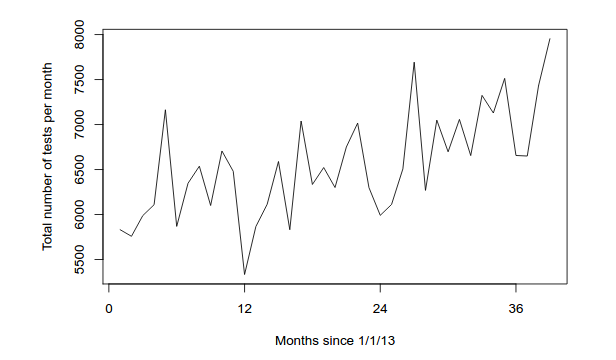
\includegraphics[scale=0.50]{Fig1.png}
\caption{}
\label{}
\end{figure}

Of note, it seems to be both a seasonal effect over the months within a year, and a general increase over years.  The use of an Analysis of Variance (ANOVA) procedure supports this interpretation of the results.\\

\begin{figure}[htp]
\centering
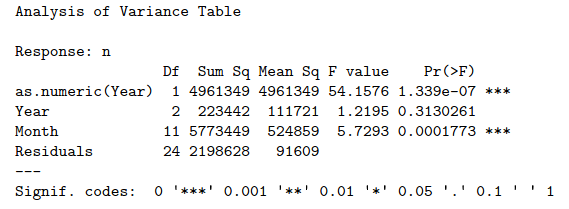
\includegraphics[scale=0.50]{fig2.png}
\caption{}
\label{}
\end{figure}

The above table (figure 2) shows that the impact of year can be summarised as a straight line effect, while we have a cyclic pattern over the months. Any departure from this would constitute an unusual increase in total workload since the introduction of RenalQ. We use a standard control chart for individuals to search for exceptional results. The control limits on the plot are calculated using the data from before the introduction of RenalQ and are at two (shown in orange) and three (shown in red) standard deviations from the centre line (see figure 3).\\

\begin{figure}[htp]
\centering
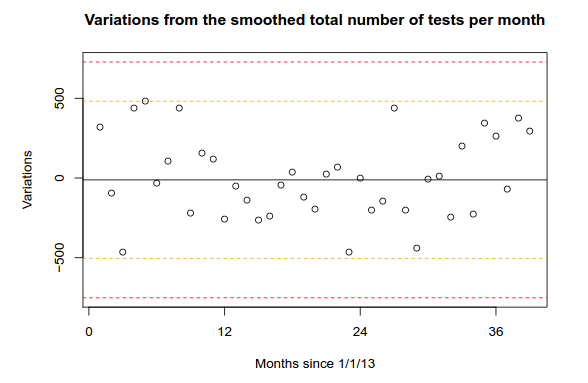
\includegraphics[scale=0.50]{fig4.png}
\caption{}
\label{}
\end{figure}

There are no serious departures (outside three standard deviation limits) from the expected for the volume of the renal function tests performed. We do need to condition this assessment on our concern that the totality of test volumes has not been provided for earlier years of this investigation. \\

Even though the total number of tests is growing, it is worth seeing if the mix of tests is changing at all. We have used a $\chi^2$ test to see if the counts of tests yielding different eGFR values is changing over time. The eGFR values have been put into five categories using cut-offs of 15, 30, 60, and 90.\\

\begin{figure}[htp]
\centering
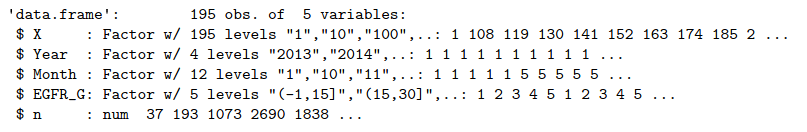
\includegraphics[scale=0.50]{fig5.png}
\caption{}
\label{}
\end{figure}

The test has a $\chi^2$ value of 3175.89 (p=0, df=152) which means there is a change in the pattern of testing over time for the five categories.\\

\begin{figure}[htp]
\centering
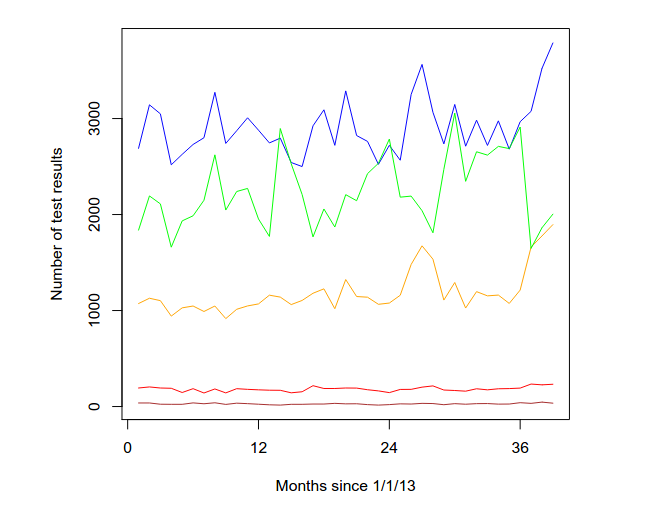
\includegraphics[scale=0.50]{fig6.png}
\caption{}
\label{}
\end{figure}

It is difficult to see any growth in the number of tests being conducted for patients whose eGFR is between 60 and 90 (shown in blue) and above 90 (shown in green). The patient groups of greatest interest are those with eGFR between 30 and 60 (shown in orange) and between 15 and 30 (shown in red).\\

In the following analysis, the data for 2013 has been added back in and we have evaluated every value of eGFR instead of grouped eGFR values.The next  model  used to identify the statistically significant factors affecting the time between successive renal function tests allows for only the level of renal function for each patient (as measured by their eGFR), and whether that test was analyzed using the RenalQ system. In addition, the combination of these two effects has also been incorporated in the model. The regression model for this model yields  the following summary of effects and their statistical significance. These show that there has been a statistically significant reduction in the time of next test for patients with serious renal impairment, of sufficent magnitude a logrithmic scale is required to visualise the effect.\\

\begin{figure}[htp]
\centering
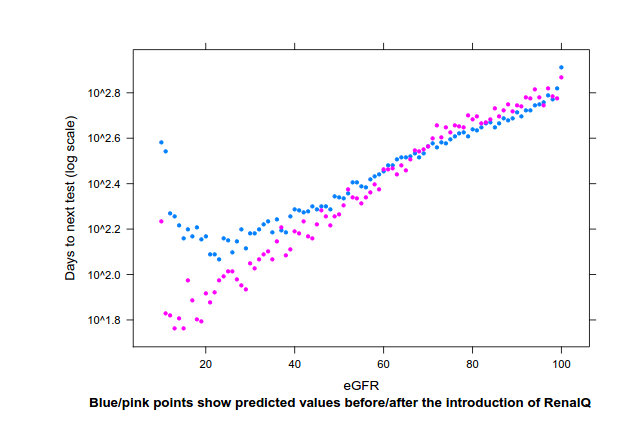
\includegraphics[scale=0.50]{FigCritical.png}
\caption{}
\label{}
\end{figure}

The pattern of change in time to next test is in accordance with our projections. We were expected the result of a decrease between tests for patients with serious renal impairment. The middle zone of mild renal impairment fulfilled our expectation of no change. Only time will tell if the expected increase in time between tests for those patients with mild or no renal impairment occurs. Given the time between tests in this group of patients is expected to be measured in years, it will be some time before if our hypothesis is confirmed. The clinical benefit of RenalQ is already established through the reduction or optimization between tests for those patients with moderate to severe renal impairment. Any financial benefit will only occur with reduction in testing frequency in thos with mild or no renal impairment.

\section{Conclusions}
The management of laboratory results in general and renal function tests, in particular, are significant issues. The combination of an aging population and an increasing incidence of predisposing illness such as diabetes means renal disease will become even more important in the future. For the practitioner, renal function tests need to be interpreted within the patient's context. The same result will mean different things for different patients. With time frames measured in measured in months or years for chronic renal impairment, losing contextual awareness of the significance and interpretation of any one result in a busy practice borders on the inevitable. The consequences for both the patient and the affordability of health care is significant.\\

RenalQ was developed to solve these issues, as characterised by the two case examples. Both of these cases were analysised by RenalQ. In both situations RenalQ was able to alert the clinician, earlier than existing human only processes. Considering the impact at the district wide level, RenalQ has statistically significantly reduced the time between tests for patients with moderate to severe renal impairment. RenalQ is therefore able to make an impact at the individual and district level. \\

It could be argued that clinicians are ignoring the RenalQ analysis. So RenalQ might not be the causal agent for this dramatic change in behaviour coincidental with the release of the application into the "wild". The counter is that RenalQ provides individualized, situational assistance to the clinician at the point of decision-making, so creating an opportunity for patient to receive timely, appropriate care. This opportunity is independent of whether the clinician is in concordance with RenalQ or not. RenalQ flagged the patient's result as benefiting from clinician review. That is the success of RenalQ.  The application changes clinical outcomes by selectively focusing attention on where clinical attention is of most benefit to the patient.  Additionally in some situations, where the clinician interpreting the result might not be familiar with the patient or the clinical situation, RenalQ provides further assistance through suggestions. \\ 

As an innovation methodology the development of RenalQ took only four years from conceptualization to being able to demonstrate statistically significant patient benefit. Typically the time frame for the successful implementation of effective innovation into clinical practice is 17 years \citep{morris2011answer}. Being the author's first project there was a steep learning. Equally having traversed the learning curve once, the next application should have an even shorter time frame than four years from conceptualization to delivering clinical benefits. \\

Part of the success of this project was due to the use of the R statistical language \citep{rstat2013}. This powerful and effective language for data analysis leading to both insight and new products is a New Zealand success story. Developed by Ross Ihaka and Robert Gentleman from the University of Auckland and first released in 1994, R language now features in lists of the top ten languages used in the world. Almost unbelievably, R statistical language was developed and is maintained as an open source project that is free to use across multiple platforms. Given the explosion in the quantity of data collected, the need for smart use of resources but the development needs to occur within a tight fiscal envelope, R statistical language represents a compelling option for future developments. \\

RenalQ is a first generation cognitive computing application, and has demonstrated the potential of this approach. To date, RenalQ has successfully improved the testing of patients most in need due to moderate to severe renal disease. Time will tell if RenalQ decreases testing rates in patients with mild or no renal impairment. This far larger group is where any potential cost savings will occur. If this does occur then RenalQ might be considered as an exemplar of the role of technology intended in the New Zealand Health Strategy (2016).



\bibliographystyle{plain}
\bibliography{NZMJ}

\end{document}
